% Created 2023-03-18 sáb 18:38
% Intended LaTeX compiler: pdflatex
\documentclass[aspectratio=169, usenames,svgnames,dvipsnames]{beamer}
\usepackage[utf8]{inputenc}
\usepackage[T1]{fontenc}
\usepackage{graphicx}
\usepackage{longtable}
\usepackage{wrapfig}
\usepackage{rotating}
\usepackage[normalem]{ulem}
\usepackage{amsmath}
\usepackage{amssymb}
\usepackage{capt-of}
\usepackage{hyperref}
\usepackage{color}
\usepackage{listings}
\usepackage{mathpazo}
\usepackage{gensymb}
\usepackage{amsmath}
\usepackage{diffcoeff}
\usepackage{steinmetz}
\usepackage{mathtools}
\usepackage{fancyvrb}
\DefineVerbatimEnvironment{verbatim}{Verbatim}{fontsize=\tiny, formatcom = {\color{black!70}}}
\bibliographystyle{plain}
\usepackage{siunitx}
\sisetup{per-mode=symbol}
\sisetup{output-decimal-marker={,}}
\DeclareSIUnit{\watthour}{Wh}
\DeclareSIUnit{\wattpeak}{Wp}
\DeclareSIUnit{\watthour}{Wh}
\DeclareSIUnit{\amperehour}{Ah}
\usepackage{steinmetz}
\hypersetup{colorlinks=true, linkcolor=Blue, urlcolor=Blue}
\usepackage[symbol, perpage]{footmisc}
\parskip=5pt
\usetheme{Boadilla}
\usecolortheme{rose}
\usefonttheme{serif}
\author{\href{https://oscarperpinan.github.io}{Oscar Perpiñán Lamigueiro}}
\date{}
\title{Sombras y Ocupación de Terreno}
\subtitle{Energía Solar Fotovoltaica}
\institute[UPM]{Universidad Politécnica de Madrid}
\setbeamercolor{alerted text}{fg=blue!50!black} \setbeamerfont{alerted text}{series=\bfseries}
\AtBeginSubsection[]{\begin{frame}[plain]\tableofcontents[currentsubsection,sectionstyle=show/hide,subsectionstyle=show/shaded/hide]\end{frame}}
\AtBeginSection[]{\begin{frame}[plain]\tableofcontents[currentsection,hideallsubsections]\end{frame}}
\beamertemplatenavigationsymbolsempty
\setbeamertemplate{footline}[frame number]
\setbeamertemplate{itemize items}[triangle]
\setbeamertemplate{enumerate items}[circle]
\setbeamertemplate{section in toc}[circle]
\setbeamertemplate{subsection in toc}[circle]
\hypersetup{
 pdfauthor={\href{https://oscarperpinan.github.io}{Oscar Perpiñán Lamigueiro}},
 pdftitle={Sombras y Ocupación de Terreno},
 pdfkeywords={},
 pdfsubject={},
 pdfcreator={Emacs 28.2 (Org mode 9.6)}, 
 pdflang={Spanish}}
\begin{document}

\maketitle

\section{Sistemas estáticos}
\label{sec:org899e005}

\begin{frame}[label={sec:orgd66c2a6}]{Sombras entre filas}
\begin{center}
\includegraphics[width=.9\linewidth]{../figs/SombraEstaticaInclinado2.pdf}
\end{center}
\end{frame}

\begin{frame}[label={sec:org7135af8}]{Sombras entre filas}
\begin{itemize}
\item Suele establecerse un objetivo de \alert{4 horas de sol en torno al mediodía del solsticio de invierno libres de sombra}.

\item La longitud de la sombra de un obstáculo se mide con:$$d=\frac{h}{\tan\gamma_{s}}$$

\item En el mediodía del solsticio de invierno
\end{itemize}
$$\gamma_{s}=90-23.45-\phi\simeq67-\phi$$ 

\begin{itemize}
\item Para 2 horas antes y después:
\end{itemize}
$$d_{min}=\frac{h}{\tan(61\degree-\phi)}$$
\end{frame}
\begin{frame}[label={sec:orgdbbc8be}]{Separación entre filas}
\begin{columns}
\begin{column}{0.65\columnwidth}
\begin{center}
\includegraphics[angle=90,height=0.7\textheight]{../figs/AbacoSombraEst_Ene10.pdf}
\end{center}
\end{column}



\begin{column}{0.35\columnwidth}
\begin{center}
\includegraphics[height=0.3\textheight]{../figs/DimensionesSeguidorSombra.pdf}
\end{center}

\[
W=\infty\]
\[
  ROT=D/L
\]
\[
  GCR=L/D
\]
\end{column}
\end{columns}
\end{frame}


\section{Sistemas de seguimiento 2X}
\label{sec:orgf539ece}


\begin{frame}[label={sec:orga27a33a}]{Separación de seguidores Doble Eje}
\begin{center}
\includegraphics[height=0.45\textheight]{../figs/Sombras2X.pdf}
\end{center}

\begin{columns}
\begin{column}{0.6\columnwidth}
\begin{center}
\includegraphics[height=0.35\textheight]{../figs/DimensionesSeguidorSombra.pdf}
\end{center}
\end{column}

\begin{column}{0.4\columnwidth}
$$ROT=\frac{L_{ns}\cdot L_{eo}}{L \cdot W}$$
$$GCR=\frac{L \cdot W}{L_{ns}\cdot L_{eo}}$$
$$E_{ac}=f(ROT)??$$
\end{column}
\end{columns}
\end{frame}

\begin{frame}[label={sec:orgc68b1c2}]{Radiación promedio}
$$G_{ef, av} = 1/24 \cdot \left( 10 \cdot G_{ef,0} + 5 \cdot G_{ef,A} + G_{ef,B} + 2 \cdot G_{ef,C} + G_{ef,D} + 5 \cdot G_{ef,E} \right)$$

\begin{columns}
\begin{column}{0.4\columnwidth}
\begin{center}
\includegraphics[height=0.7\textheight]{../figs/plantConfiguration.pdf}
\end{center}
\end{column}

\begin{column}{0.6\columnwidth}
\begin{center}
\includegraphics[width=.9\linewidth]{../figs/6trackers.pdf}
\end{center}
\end{column}
\end{columns}
\end{frame}


\begin{frame}[label={sec:orgc6cb136}]{Separación de Seguidores Doble Eje}
\begin{columns}
\begin{column}{0.3\columnwidth}
$$b=\frac{L}{W}=0.475$$

$$ROT=\frac{L_{ns}\cdot L_{eo}}{L \cdot W}$$
$$GCR=\frac{L \cdot W}{L_{ns}\cdot L_{eo}}$$
\end{column}

\begin{column}{0.7\columnwidth}
\begin{center}
\includegraphics[height=0.9\textheight]{../figs/AbacoSeguidor2X_Ene10.pdf}
\end{center}
\end{column}
\end{columns}
\end{frame}


\section{Seguidores de eje horizontal NS}
\label{sec:orgd77fc4e}

\begin{frame}[label={sec:org5e5cb13}]{Separación de Seguidores Eje Horizontal}
\begin{center}
\includegraphics[height=0.9\textheight]{../figs/SombrasHoriz.pdf}
\end{center}

$$W=\infty$$ $$ROT=L_{eo}/L$$
\end{frame}

\begin{frame}[label={sec:org2307743}]{Separación de Seguidores Horizontal N-S}
\begin{center}
\includegraphics[angle=90,height=0.9\textheight]{../figs/AbacoSeguidorHorizSombra_Ene10.pdf}
\end{center}
\end{frame}

\begin{frame}[label={sec:org2ff6c42}]{Backtracking}
\begin{itemize}
\item El \alert{sombreado} en un generador puede producir problemas por el efecto
de \alert{punto caliente}.

\item En seguidores de eje horizontal se puede \alert{evitar la incidencia de
sombras} en cualquier instante mediante el \guillemotleft{}\alert{backtracking}\guillemotright{}:

\begin{itemize}
\item Al \alert{amanecer} el seguidor está en posición \alert{horizontal}.

\item Según avanza el día el seguidor gira en \alert{sentido contrario al
movimiento solar para evitar las sombras}.

\item En un determinado momento se cruza con el sol y puede continuar el
movimiento \guillemotleft{}convencional\guillemotright{}.

\item En un instante de la tarde debe volver a cambiar el sentido hasta
la \alert{horizontal en la noche}.
\end{itemize}
\end{itemize}
\end{frame}

\begin{frame}[label={sec:org1bb3747}]{Backtracking}
\begin{center}
\includegraphics[height=0.9\textheight]{../figs/BackTracking.pdf}
\end{center}
\end{frame}

\begin{frame}[label={sec:orgd07f329}]{Separación con backtracking}
\begin{center}
\includegraphics[angle=90,height=0.9\textheight]{../figs/AbacoHorizBT_Ene10.pdf}
\end{center}
\end{frame}

\begin{frame}[label={sec:org085f889}]{Limitación de ángulo}
\begin{itemize}
\item Es habitual limitar el ángulo de inclinación a valores máximos alrededor de 70° por motivos estructurales (protección frente al viento)

\item Implica un desvio de los seguidores de su posición óptima.

\begin{itemize}
\item Sombras más cortas que en el caso teórico (red más densa).

\item Reducción en la energía generada por incidencia no perpendicular
\end{itemize}
\end{itemize}
\end{frame}

\section{Elección de separaciones}
\label{sec:org7580be2}


\begin{frame}[label={sec:org4b009ea}]{Elección de separaciones}
La \alert{separación óptima} entre elementos (seguidores o estructuras
estáticas) es aquella que conduce al \alert{mínimo valor del coste de la
energía} producida por el sistema.

Al aumentar la separación:

\begin{itemize}
\item Disminuyen las \alert{pérdidas por sombreado mutuo} (aumenta la
productividad del

\item Aumentan:

\begin{itemize}
\item los \alert{costes relacionados con el área ocupada} por unidad de
potencia.
\item los \alert{costes relacionados con los elementos de unión entre estructuras} (cableado, canalizaciones, zanjas).
\end{itemize}
\end{itemize}
\end{frame}

\begin{frame}[label={sec:org3871e96}]{Elección de separaciones}
\begin{itemize}
\item Esta separación óptima \alert{depende} de las \alert{estructuras elegidas} y de
las \alert{condiciones económicas} de los elementos.

\item La separación finalmente elegida debe \alert{tomar en consideración las
condiciones del terreno} (fronteras, irregularidades, vaguadas, etc.)
\end{itemize}
\end{frame}

\begin{frame}[label={sec:orgf783d3b}]{Ocupación óptima}
\begin{columns}
\begin{column}{0.6\columnwidth}
\begin{center}
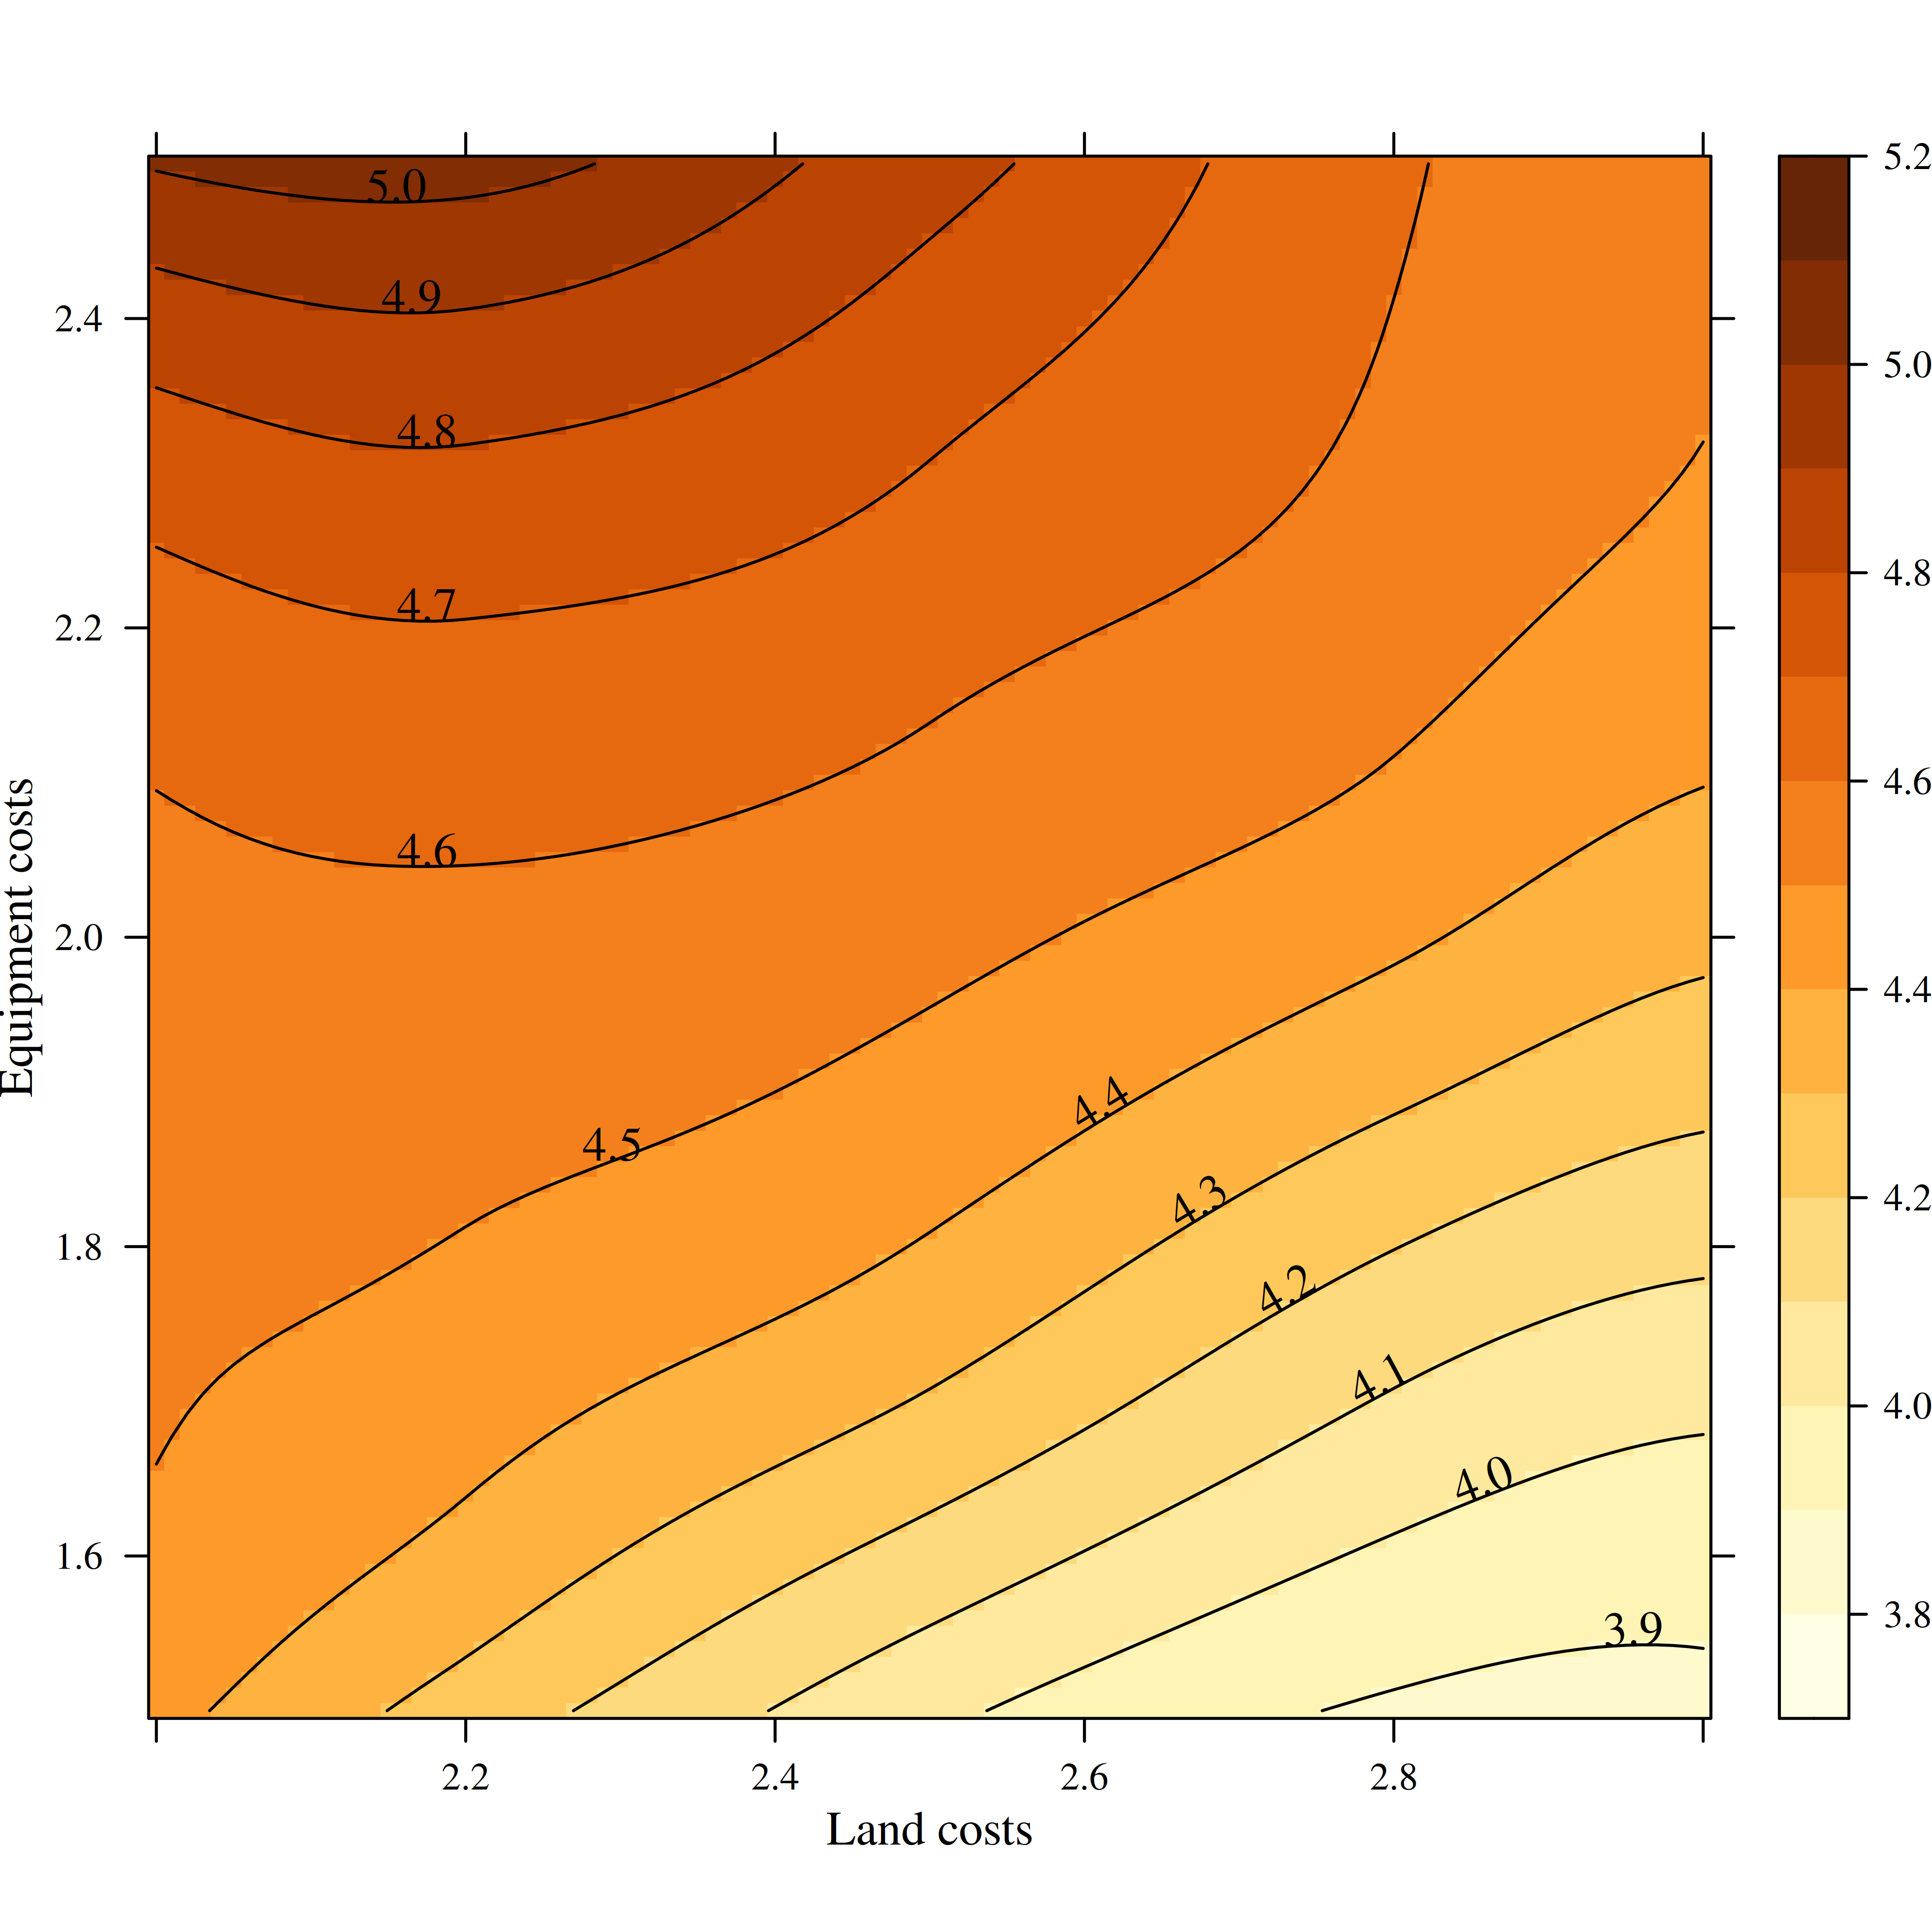
\includegraphics[height=0.9\textheight]{../figs/GRRoptim.png}
\end{center}
\end{column}

\begin{column}{0.4\columnwidth}
\begin{itemize}
\item Coste Energía
$$C_E = \frac{C_P}{E_{AC}}$$
\item Coste Sistema
$$C_p = C_c + C_A + C_{PV}$$

\item \(C_{PV}\) entre \(\SI{1.5}{\text{\texteuro}\per\watt}\) y \(\SI{2.5}{\text{\texteuro}\per\watt}\)

\item \(C_A\) entre \(\SI{2}{\text{\texteuro}\per\meter\squared}\) y \(\SI{3}{\text{\texteuro}\per\meter\squared}\)
\end{itemize}
\end{column}
\end{columns}
\end{frame}

\begin{frame}[label={sec:org101a349}]{Separaciones y coste de la energía}
\begin{center}
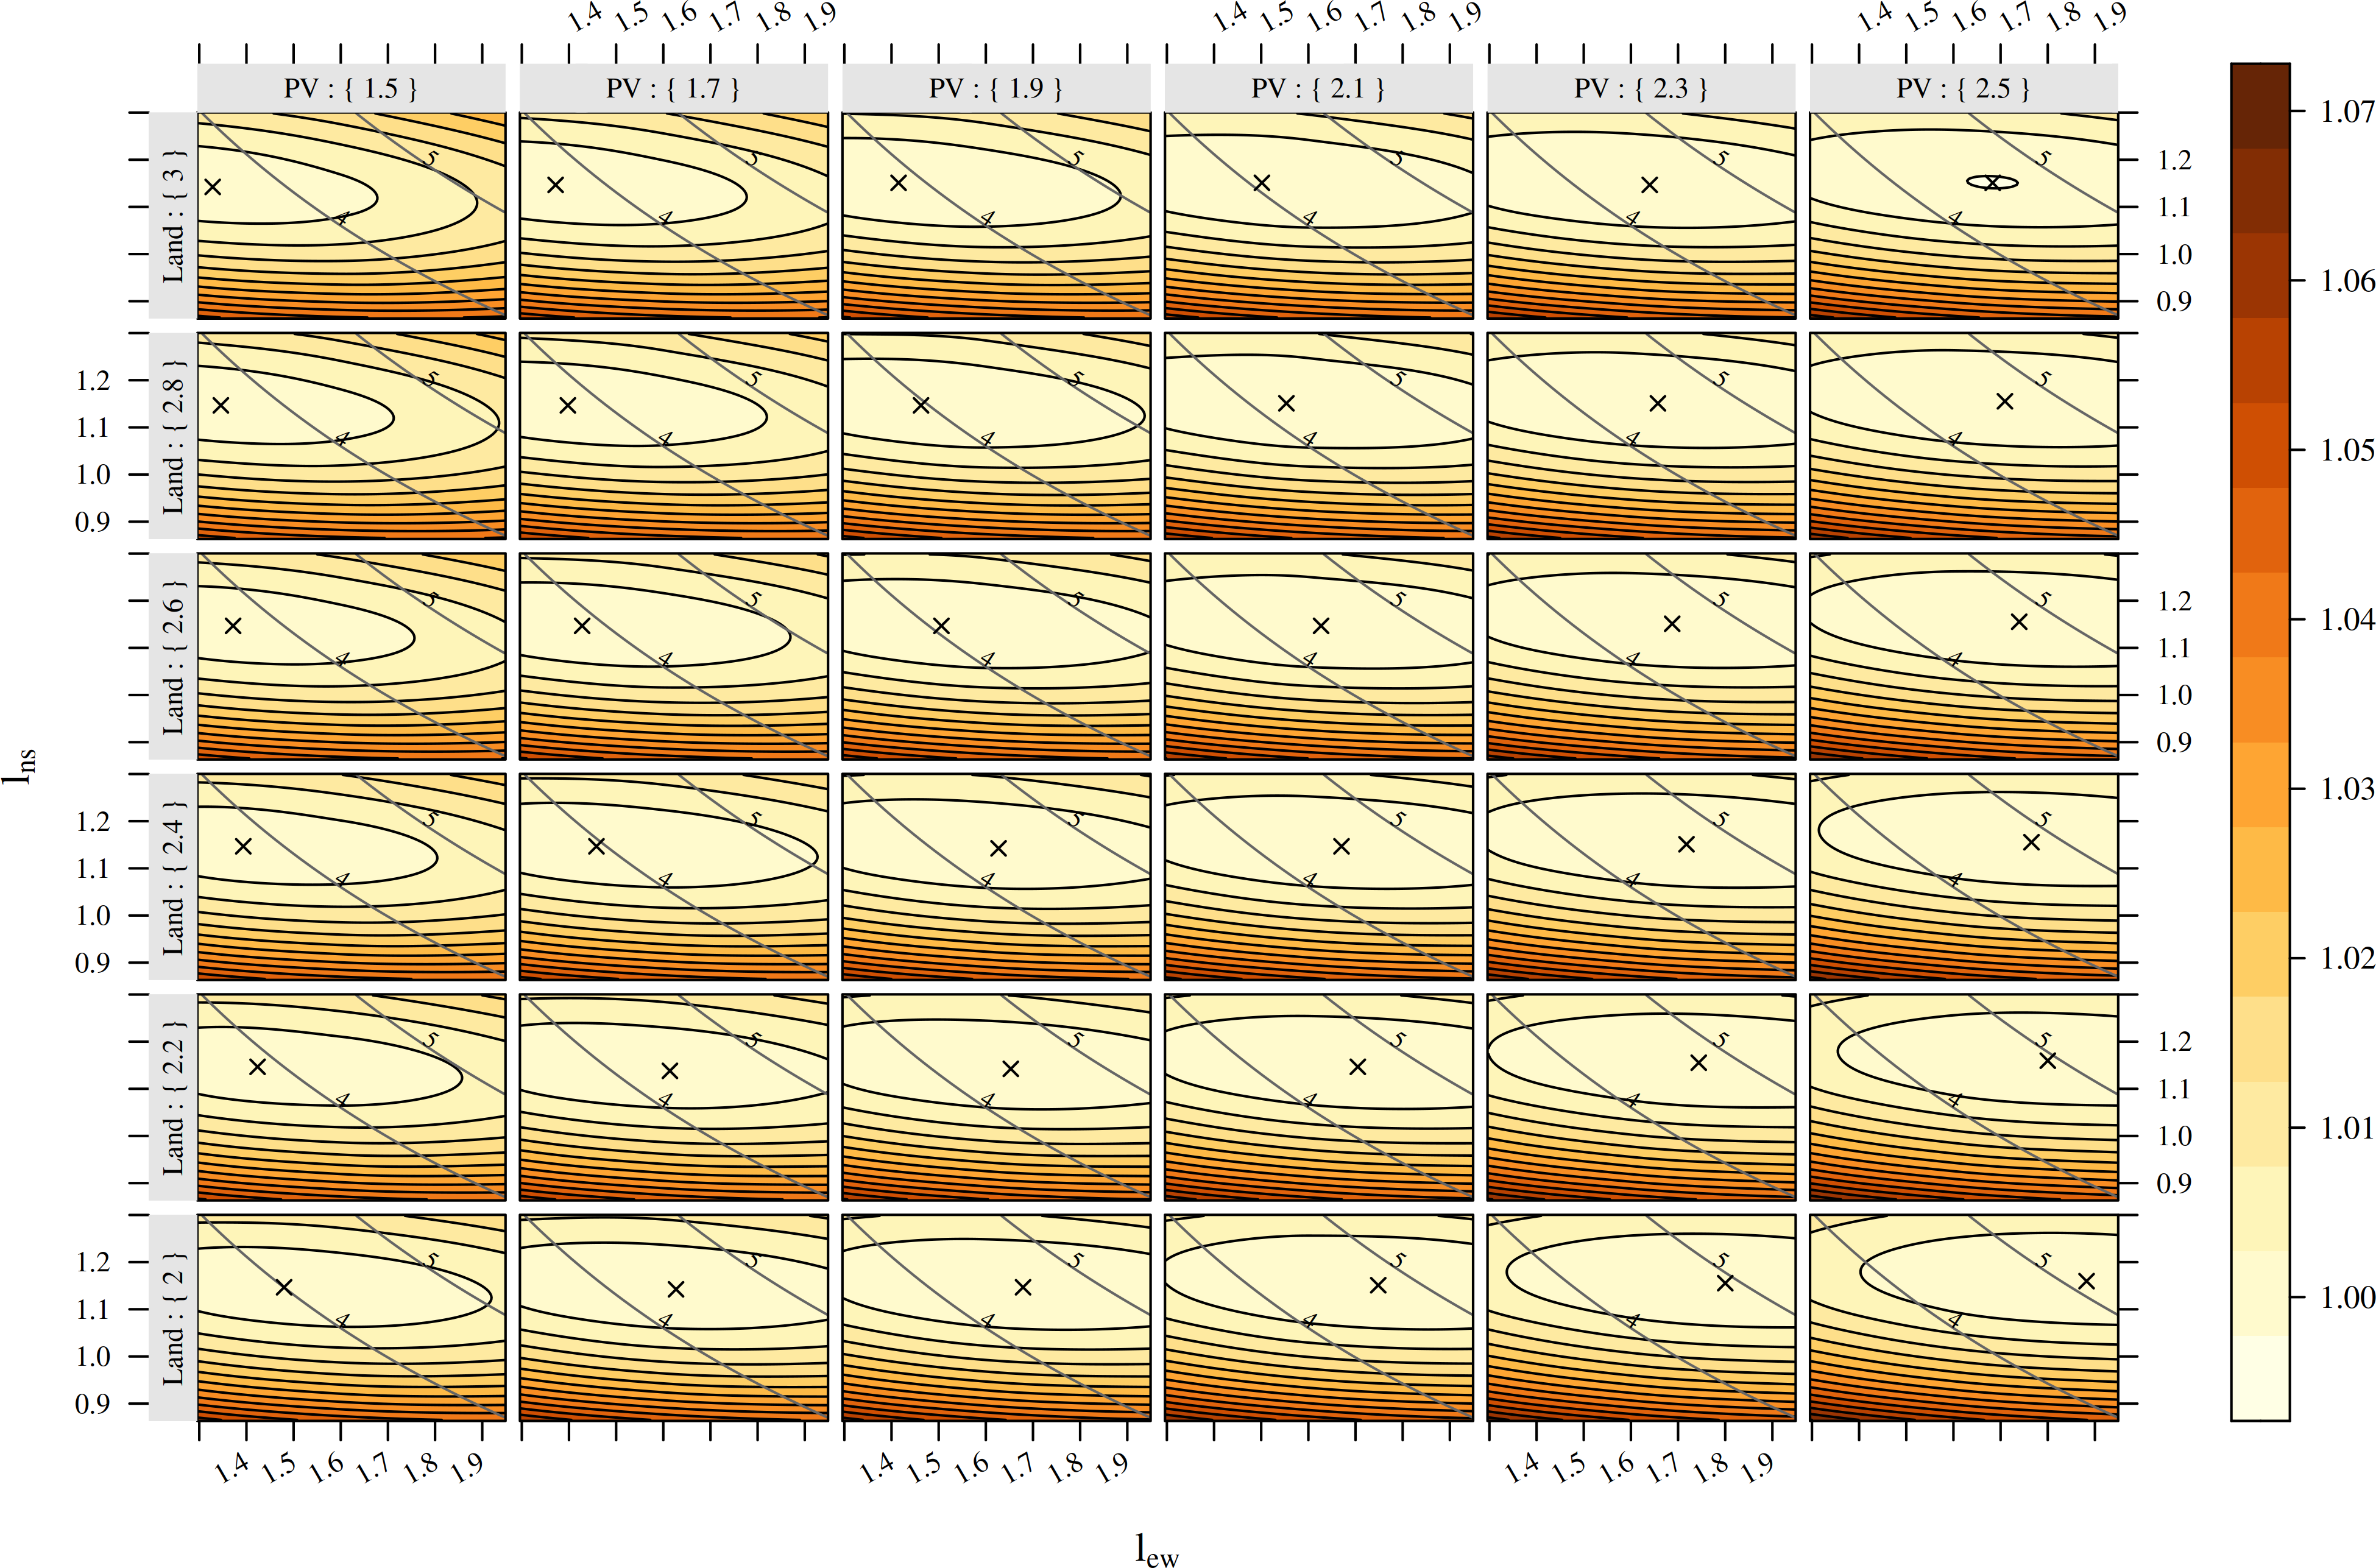
\includegraphics[height=0.9\textheight]{../figs/matrixGRR.png}
\end{center}
\end{frame}
\end{document}